\documentclass[tikz,border=2pt,11pt]{standalone}
\usetikzlibrary{matrix}
\usetikzlibrary{positioning}
\usetikzlibrary{arrows.meta}
\usetikzlibrary{calc}
\usetikzlibrary{fit}
\usetikzlibrary{backgrounds}
\usetikzlibrary{decorations.pathreplacing}
\usepackage{amsmath}
\usepackage{amssymb}
\usepackage{tikz}
\newcommand{\C}{\mathbb C}
\newcommand{\R}{\mathbb R}
\newcommand{\N}{\mathbb N}
\newcommand{\Id}{I}
\newcommand{\eps}{\varepsilon}
\DeclareMathOperator{\GL}{GL}
\DeclareMathOperator{\Mat}{Mat}
\DeclareMathOperator{\diag}{diag}
\DeclareMathOperator{\rank}{rank}
\DeclareMathOperator{\tr}{tr}
\DeclareMathOperator{\supp}{supp}
\DeclareMathOperator{\nnz}{nnz}
\DeclareMathOperator{\im}{im}
\DeclareMathOperator{\Span}{span}
\DeclareMathOperator{\poly}{poly}
\begin{document}
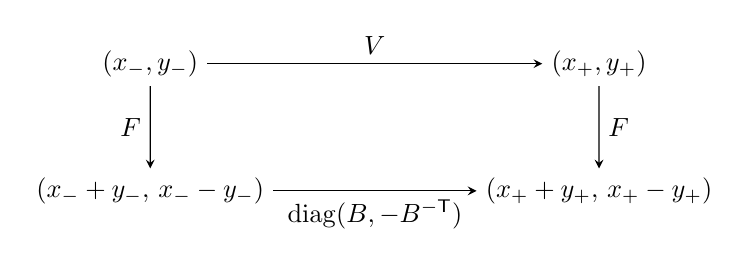
\begin{tikzpicture}[>=stealth, every node/.style={align=center},
                    scale=0.95, transform shape]
 \node (a) at (0,1.5) {$ (x_-,y_-) $};
 \node (b) at (6,1.5) {$ (x_+,y_+) $};
 \node (c) at (0,-0.2) {$ (x_-+y_-,\,x_--y_-) $};
 \node (e) at (6,-0.2) {$ (x_++y_+,\,x_+-y_+) $};
 \draw[->] (a) -- node[above] {$V$} (b);
 \draw[->] (a) -- node[left] {$F$} (c);
 \draw[->] (b) -- node[right] {$F$} (e);
 \draw[->] (c) -- node[below] {$\diag(B,-B^{-\mathsf T})$} (e);
\end{tikzpicture}
\end{document}
